\chapter{Controllo degli accessi}

Il controllo degli accessi è un elemento centrale nella sicurezza 
informatica. È il \textbf{meccanismo} che definisce una \textbf{politica 
di sicurezza} per la quale si decide quali utenti possano accedere o 
meno ad una risorsa.

\noindent Si basa su tre principi fondamentali:
\begin{itemize}
    \item \textbf{Autenticazione:} verifica che le credenziali fornite 
    siano valide 
    \item \textbf{Autorizzazione:} concessione di un permesso ad un'entità
    affinché possa accedere ad una risorsa del sistema 
    \item \textbf{Auditing:} verifica delle attività e dei registri di 
    sistema
\end{itemize}

\begin{figure}[H]
    \centering
    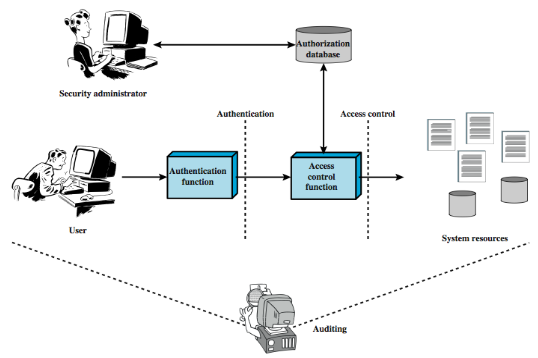
\includegraphics[width=1\linewidth]{chapters/3/images/ac.png}
\end{figure}